\section{Experiments}
\label{sec:results}

\subsection{Setup}

\paragraph{Benchmarks.}
We evaluate on \textbf{TOFU} \citep{maini2024tofu} (fictitious QA, Llama-3.2-1B/3B, 3 forget splits),
\textbf{MUSE Books/News} \citep{shi2025muse} (Harry Potter / BBC articles, Llama-2-7B),
and \textbf{KnowUndo} \citep{tian2024knowundo} (copyright/privacy, Llama-2-7B-chat).
All results are 5-fold (seeds 42/123/456/789/1024) unless noted.

\paragraph{Composite scores.} We report harmonic means that penalize imbalance across axes:
\begin{itemize}[leftmargin=*, topsep=2pt, itemsep=0pt]
    \item TOFU: $\text{HM} = \text{hmean}(\text{MU},\; 1{-}\text{Prob},\; 1{-}\text{ROUGE})$
    \item MUSE: $\text{HM} = \text{hmean}(1{-}\text{fk},\; 1{-}\text{vm},\; \text{rk})$
    \item KnowUndo: $\text{HM} = \text{hmean}(1{-}\text{fgt\_R},\; \text{ret\_R},\; \text{MMLU})$
    \item LLM Judge: $\text{HM}_\text{J} = \text{hmean}(1{-}\text{FL}/2,\; \text{RA}/2,\; \text{rRQ}/2)$
\end{itemize}

\paragraph{LLM judge.} We use Claude Opus~4.7 to score generations on a 0--2 scale: Forget Leakage (FL$\downarrow$), Retain Accuracy (RA$\uparrow$), and retain Response Quality (rRQ$\uparrow$). Token-level metrics like ROUGE miss subtle leakage that a judge can detect from semantic content.

%% ============================================================
\subsection{TOFU (Llama-3.2-1B-Instruct)}
\label{sec:tofu_1b}
%% ============================================================

\begin{table*}[t!]
\centering
\small
\caption{TOFU 1B full results (5 seeds). HM = hmean(MU, 1$-$Prob, 1$-$ROUGE). Best in \textbf{bold}.}
\label{tab:tofu_1b_full}
\resizebox{\textwidth}{!}{%
\begin{tabular}{@{}l|cccc|cccc|cccc@{}}
\toprule
& \multicolumn{4}{c|}{Forget 1\%} & \multicolumn{4}{c|}{Forget 5\%} & \multicolumn{4}{c}{Forget 10\%} \\
Method & MU$\uparrow$ & Prob$\downarrow$ & ROUGE$\downarrow$ & HM$\uparrow$ & MU$\uparrow$ & Prob$\downarrow$ & ROUGE$\downarrow$ & HM$\uparrow$ & MU$\uparrow$ & Prob$\downarrow$ & ROUGE$\downarrow$ & HM$\uparrow$ \\
\midrule
Gold & .597 & .166 & .414 & .655 & .599 & .127 & .383 & .676 & .591 & .116 & .379 & .677 \\
\midrule
GradAscent & .596$_{\pm.00}$ & .477$_{\pm.01}$ & .456$_{\pm.01}$ & .553$_{\pm.01}$ & .008$_{\pm.01}$ & .003$_{\pm.01}$ & .112$_{\pm.08}$ & .022$_{\pm.04}$ & .000$_{\pm.00}$ & .000$_{\pm.00}$ & .001$_{\pm.00}$ & .000$_{\pm.00}$ \\
GradDiff & .581$_{\pm.01}$ & .421$_{\pm.04}$ & .464$_{\pm.02}$ & .564$_{\pm.01}$ & .453$_{\pm.00}$ & .073$_{\pm.00}$ & .375$_{\pm.01}$ & .614$_{\pm.01}$ & .435$_{\pm.00}$ & .047$_{\pm.00}$ & .339$_{\pm.01}$ & .617$_{\pm.00}$ \\
NPO & .596$_{\pm.00}$ & .474$_{\pm.01}$ & .438$_{\pm.02}$ & .560$_{\pm.01}$ & .454$_{\pm.01}$ & .245$_{\pm.01}$ & .308$_{\pm.01}$ & .603$_{\pm.01}$ & .393$_{\pm.03}$ & .213$_{\pm.01}$ & .210$_{\pm.01}$ & .590$_{\pm.02}$ \\
SimNPO & .594$_{\pm.00}$ & .858$_{\pm.01}$ & .734$_{\pm.02}$ & .240$_{\pm.01}$ & .596$_{\pm.00}$ & .848$_{\pm.00}$ & .741$_{\pm.01}$ & .248$_{\pm.00}$ & .597$_{\pm.00}$ & .842$_{\pm.00}$ & .734$_{\pm.01}$ & .255$_{\pm.00}$ \\
RMU & .557$_{\pm.00}$ & .414$_{\pm.01}$ & .415$_{\pm.00}$ & .576$_{\pm.00}$ & .546$_{\pm.00}$ & .369$_{\pm.01}$ & .423$_{\pm.01}$ & .583$_{\pm.00}$ & .572$_{\pm.00}$ & .106$_{\pm.02}$ & .322$_{\pm.01}$ & .691$_{\pm.01}$ \\
BLURNPO & .598$_{\pm.00}$ & .676$_{\pm.01}$ & .588$_{\pm.02}$ & .417$_{\pm.01}$ & .518$_{\pm.02}$ & .475$_{\pm.07}$ & .407$_{\pm.05}$ & .541$_{\pm.04}$ & .089$_{\pm.14}$ & .087$_{\pm.04}$ & .253$_{\pm.09}$ & .154$_{\pm.20}$ \\
PDU & .602$_{\pm.00}$ & .186$_{\pm.01}$ & .313$_{\pm.01}$ & .690$_{\pm.01}$ & .588$_{\pm.00}$ & .073$_{\pm.02}$ & .214$_{\pm.03}$ & .740$_{\pm.01}$ & .592$_{\pm.00}$ & .004$_{\pm.00}$ & .065$_{\pm.01}$ & .797$_{\pm.00}$ \\
\midrule
\method & .599$_{\pm.00}$ & \textbf{.002}$_{\pm.00}$ & \textbf{.038}$_{\pm.00}$ & \textbf{.808}$_{\pm.00}$ & .597$_{\pm.00}$ & \textbf{.015}$_{\pm.00}$ & \textbf{.054}$_{\pm.01}$ & \textbf{.800}$_{\pm.00}$ & .593$_{\pm.01}$ & \textbf{.009}$_{\pm.00}$ & \textbf{.039}$_{\pm.01}$ & \textbf{.803}$_{\pm.00}$ \\
\bottomrule
\end{tabular}}
\end{table*}

\begin{table*}[t!]
\centering
\small
\caption{LLM Judge on TOFU 1B (5 seeds, Claude Opus~4.7). Best in \textbf{bold}.}
\label{tab:tofu_1b_judge}
\resizebox{\textwidth}{!}{%
\begin{tabular}{@{}l|cccc|cccc|cccc@{}}
\toprule
& \multicolumn{4}{c|}{Forget 1\%} & \multicolumn{4}{c|}{Forget 5\%} & \multicolumn{4}{c}{Forget 10\%} \\
Method & FL$\downarrow$ & RA$\uparrow$ & rRQ$\uparrow$ & HM$_\text{J}$$\uparrow$ & FL$\downarrow$ & RA$\uparrow$ & rRQ$\uparrow$ & HM$_\text{J}$$\uparrow$ & FL$\downarrow$ & RA$\uparrow$ & rRQ$\uparrow$ & HM$_\text{J}$$\uparrow$ \\
\midrule
GradAscent & 1.11$_{\pm.05}$ & 1.66$_{\pm.01}$ & 1.99$_{\pm.00}$ & .674$_{\pm.02}$ & 0.07$_{\pm.07}$ & 0.10$_{\pm.09}$ & 0.51$_{\pm.43}$ & .117$_{\pm.10}$ & 0.00$_{\pm.00}$ & 0.00$_{\pm.00}$ & 0.00$_{\pm.00}$ & .000$_{\pm.00}$ \\
GradDiff & 1.21$_{\pm.07}$ & 1.54$_{\pm.04}$ & 1.97$_{\pm.01}$ & .620$_{\pm.02}$ & 0.65$_{\pm.03}$ & 1.01$_{\pm.01}$ & 1.68$_{\pm.01}$ & .643$_{\pm.00}$ & 0.46$_{\pm.01}$ & 0.91$_{\pm.02}$ & 1.53$_{\pm.04}$ & .625$_{\pm.01}$ \\
NPO & 1.05$_{\pm.08}$ & 1.67$_{\pm.01}$ & 1.99$_{\pm.00}$ & .696$_{\pm.03}$ & 0.44$_{\pm.02}$ & 1.14$_{\pm.05}$ & 1.89$_{\pm.02}$ & .731$_{\pm.01}$ & 0.44$_{\pm.02}$ & 0.94$_{\pm.07}$ & 1.82$_{\pm.04}$ & .665$_{\pm.03}$ \\
SimNPO & 1.76$_{\pm.03}$ & 1.66$_{\pm.01}$ & 1.99$_{\pm.00}$ & .288$_{\pm.03}$ & 1.58$_{\pm.01}$ & 1.69$_{\pm.01}$ & 1.99$_{\pm.00}$ & .435$_{\pm.01}$ & 1.58$_{\pm.02}$ & 1.72$_{\pm.02}$ & 1.99$_{\pm.00}$ & .435$_{\pm.02}$ \\
RMU & 0.81$_{\pm.05}$ & 1.39$_{\pm.01}$ & 1.93$_{\pm.01}$ & .721$_{\pm.01}$ & 0.72$_{\pm.04}$ & 1.36$_{\pm.02}$ & 1.91$_{\pm.01}$ & .736$_{\pm.01}$ & 0.29$_{\pm.04}$ & 1.50$_{\pm.01}$ & 1.98$_{\pm.00}$ & .854$_{\pm.01}$ \\
BLURNPO & 1.40$_{\pm.05}$ & 1.67$_{\pm.01}$ & 1.99$_{\pm.00}$ & .541$_{\pm.03}$ & 0.86$_{\pm.08}$ & 1.37$_{\pm.06}$ & 1.98$_{\pm.01}$ & .709$_{\pm.01}$ & 0.26$_{\pm.24}$ & 0.36$_{\pm.38}$ & 0.73$_{\pm.64}$ & .255$_{\pm.21}$ \\
PDU & 0.86$_{\pm.06}$ & 1.60$_{\pm.01}$ & 1.97$_{\pm.00}$ & .746$_{\pm.02}$ & 0.37$_{\pm.08}$ & 1.56$_{\pm.02}$ & 1.96$_{\pm.01}$ & .850$_{\pm.01}$ & 0.04$_{\pm.01}$ & 1.57$_{\pm.01}$ & 1.98$_{\pm.01}$ & .906$_{\pm.00}$ \\
\midrule
\method & \textbf{0.02}$_{\pm.02}$ & 1.65$_{\pm.01}$ & 1.98$_{\pm.01}$ & \textbf{.929}$_{\pm.01}$ & \textbf{0.07}$_{\pm.02}$ & 1.64$_{\pm.02}$ & 1.98$_{\pm.01}$ & \textbf{.919}$_{\pm.00}$ & \textbf{0.04}$_{\pm.02}$ & 1.63$_{\pm.02}$ & 1.98$_{\pm.00}$ & \textbf{.919}$_{\pm.01}$ \\
\bottomrule
\end{tabular}}
\end{table*}

Results on the larger 3B model (Appendix~\ref{app:tofu_full}) confirm the same pattern: \method achieves HM=0.846/0.842/0.836 across splits, with near-zero FL on the LLM judge (HM$_\text{J}$=0.970/0.962/0.965).

%% ============================================================
\subsection{MUSE Books (Llama-2-7B)}
\label{sec:muse_books}
%% ============================================================

\begin{table*}[t!]
\centering
\small
\caption{MUSE Books results (5-fold). Left: automated metrics; HM = hmean(1$-$fk, 1$-$vm, rk). Right: LLM judge (0--2 scale). Best in \textbf{bold} (excl.\ Gold).}
\label{tab:muse_books}
\begin{minipage}[t]{0.48\textwidth}
\centering
\resizebox{\textwidth}{!}{%
\begin{tabular}{@{}lcccc@{}}
\toprule
Method & fk$\downarrow$ & vm$\downarrow$ & rk$\uparrow$ & HM$\uparrow$ \\
\midrule
Gold (retrain) & .303 & .145 & .687 & .739 \\
\midrule
GradAscent & .000$_{\pm.00}$ & .000$_{\pm.00}$ & .000$_{\pm.00}$ & .000$_{\pm.00}$ \\
GradDiff & .000$_{\pm.00}$ & .000$_{\pm.00}$ & .004$_{\pm.00}$ & .011$_{\pm.01}$ \\
NPO & .303$_{\pm.02}$ & .342$_{\pm.03}$ & .574$_{\pm.02}$ & .638$_{\pm.01}$ \\
SimNPO & .238$_{\pm.02}$ & .002$_{\pm.00}$ & .600$_{\pm.01}$ & .753$_{\pm.01}$ \\
RMU & .210$_{\pm.00}$ & .113$_{\pm.01}$ & .598$_{\pm.01}$ & .738$_{\pm.00}$ \\
PDU & .139$_{\pm.01}$ & .129$_{\pm.01}$ & .372$_{\pm.01}$ & .600$_{\pm.01}$ \\
BLURNPO & .175$_{\pm.01}$ & .000$_{\pm.00}$ & .547$_{\pm.02}$ & .742$_{\pm.01}$ \\
\midrule
\method & \textbf{.089}$_{\pm.02}$ & \textbf{.000}$_{\pm.00}$ & \textbf{.638}$_{\pm.01}$ & \textbf{.818}$_{\pm.01}$ \\
\bottomrule
\end{tabular}}
\end{minipage}%
\hfill
\begin{minipage}[t]{0.48\textwidth}
\centering
\resizebox{\textwidth}{!}{%
\begin{tabular}{@{}lcccc@{}}
\toprule
Method & FL$\downarrow$ & RA$\uparrow$ & rRQ$\uparrow$ & HM$_\text{J}$$\uparrow$ \\
\midrule
\midrule
GradAscent & 0.00$_{\pm.00}$ & 0.00$_{\pm.00}$ & 0.00$_{\pm.00}$ & .000$_{\pm.00}$ \\
GradDiff & 0.00$_{\pm.00}$ & 0.04$_{\pm.02}$ & 0.01$_{\pm.01}$ & .010$_{\pm.01}$ \\
NPO & 0.91$_{\pm.03}$ & 1.28$_{\pm.03}$ & 1.61$_{\pm.01}$ & .647$_{\pm.01}$ \\
SimNPO & 0.31$_{\pm.12}$ & 1.28$_{\pm.02}$ & 1.62$_{\pm.01}$ & .753$_{\pm.02}$ \\
RMU & 0.32$_{\pm.02}$ & 1.41$_{\pm.02}$ & 1.68$_{\pm.01}$ & .791$_{\pm.00}$ \\
PDU & 0.53$_{\pm.02}$ & 0.99$_{\pm.02}$ & 1.15$_{\pm.02}$ & .586$_{\pm.01}$ \\
BLURNPO & 0.20$_{\pm.02}$ & 1.15$_{\pm.06}$ & 1.52$_{\pm.07}$ & .720$_{\pm.02}$ \\
\midrule
\method & \textbf{0.11}$_{\pm.02}$ & \textbf{1.39}$_{\pm.01}$ & \textbf{1.66}$_{\pm.02}$ & \textbf{.810}$_{\pm.01}$ \\
\bottomrule
\end{tabular}}
\end{minipage}
\end{table*}

%% ============================================================
\subsection{MUSE News (Llama-2-7B)}
\label{sec:muse_news}
%% ============================================================

\begin{table*}[t!]
\centering
\small
\caption{MUSE News results (5-fold). Left: automated metrics; best HM in \textbf{bold}. Right: LLM judge (0--2 scale).}
\label{tab:muse_news}
\begin{minipage}[t]{0.48\textwidth}
\centering
\resizebox{\textwidth}{!}{%
\begin{tabular}{@{}lcccc@{}}
\toprule
Method & fk$\downarrow$ & vm$\downarrow$ & rk$\uparrow$ & HM$\uparrow$ \\
\midrule
Gold (retrain) & .324 & .204 & .552 & .660 \\
\midrule
GradDiff & .329$_{\pm.03}$ & .043$_{\pm.02}$ & .269$_{\pm.02}$ & .479$_{\pm.02}$ \\
NPO & .517$_{\pm.02}$ & .274$_{\pm.02}$ & .435$_{\pm.01}$ & .522$_{\pm.01}$ \\
SimNPO & .628$_{\pm.01}$ & .542$_{\pm.01}$ & .513$_{\pm.01}$ & .440$_{\pm.00}$ \\
RMU & .495$_{\pm.01}$ & .267$_{\pm.01}$ & .434$_{\pm.01}$ & .531$_{\pm.00}$ \\
PDU & .525$_{\pm.02}$ & .092$_{\pm.07}$ & .508$_{\pm.04}$ & \textbf{.577}$_{\pm.01}$ \\
BLURNPO & .302$_{\pm.04}$ & .146$_{\pm.04}$ & .274$_{\pm.02}$ & .478$_{\pm.01}$ \\
\midrule
\method & .545$_{\pm.02}$ & .211$_{\pm.03}$ & .490$_{\pm.01}$ & .544$_{\pm.01}$ \\
\bottomrule
\end{tabular}}
\end{minipage}%
\hfill
\begin{minipage}[t]{0.48\textwidth}
\centering
\resizebox{\textwidth}{!}{%
\begin{tabular}{@{}lcccc@{}}
\toprule
Method & FL$\downarrow$ & RA$\uparrow$ & rRQ$\uparrow$ & HM$_\text{J}$$\uparrow$ \\
\midrule
\midrule
GradDiff & 0.58$_{\pm.02}$ & 0.79$_{\pm.04}$ & 1.16$_{\pm.14}$ & .529$_{\pm.03}$ \\
NPO & 1.20$_{\pm.03}$ & 1.05$_{\pm.02}$ & 1.58$_{\pm.01}$ & .531$_{\pm.01}$ \\
SimNPO & 1.49$_{\pm.01}$ & 1.24$_{\pm.01}$ & 1.72$_{\pm.01}$ & .447$_{\pm.01}$ \\
RMU & 1.13$_{\pm.01}$ & 1.15$_{\pm.02}$ & 1.60$_{\pm.01}$ & .565$_{\pm.00}$ \\
PDU & 0.87$_{\pm.12}$ & 1.18$_{\pm.05}$ & 1.64$_{\pm.05}$ & \textbf{.638}$_{\pm.02}$ \\
BLURNPO & 0.41$_{\pm.10}$ & 0.44$_{\pm.07}$ & 1.28$_{\pm.13}$ & .406$_{\pm.04}$ \\
\midrule
\method & 0.86$_{\pm.06}$ & 0.92$_{\pm.05}$ & 1.70$_{\pm.04}$ & .588$_{\pm.01}$ \\
\bottomrule
\end{tabular}}
\end{minipage}
\end{table*}

%% ============================================================
\subsection{KnowUndo (Llama-2-7B-chat)}
\label{sec:knowundo}
%% ============================================================

All methods 5-fold. MMLU evaluated once at seed=42, used as constant for HM computation.

\begin{table*}[t!]
\centering
\small
\caption{KnowUndo Copyright (5-fold). HM = hmean(1$-$fgt\_R, ret\_R, MMLU). Judge HM = hmean(1$-$FL/2, RA/2, rRQ/2). Opus~4.6 used as judge since Opus~4.7 safety guardrails refuse to evaluate copyrighted content. Best in \textbf{bold}.}
\label{tab:knowundo_copyright}
\resizebox{\textwidth}{!}{%
\begin{tabular}{@{}lccccc|cccc@{}}
\toprule
& \multicolumn{5}{c|}{Automated Metrics} & \multicolumn{4}{c}{LLM Judge (Opus 4.6)} \\
Method & fgt\_Acc$\downarrow$ & fgt\_R$\downarrow$ & ret\_Acc$\uparrow$ & ret\_R$\uparrow$ & HM$\uparrow$ & FL$\downarrow$ & RA$\uparrow$ & rRQ$\uparrow$ & HM$_\text{J}$$\uparrow$ \\
\midrule
FT (target) & .854 & .244 & .894 & .336 & .456 & 1.50 & 1.80 & 1.13 & .44 \\
Retrain & .666 & .205 & .890 & .343 & .468 & 0.96 & 1.79 & 1.13 & .62 \\
GradAscent & .002$_{\pm.00}$ & .000$_{\pm.00}$ & .002$_{\pm.00}$ & .000$_{\pm.00}$ & --- & 0.00$_{\pm.00}$ & 0.00$_{\pm.00}$ & 0.00$_{\pm.00}$ & --- \\
GradDiff & .002$_{\pm.00}$ & .000$_{\pm.00}$ & .642$_{\pm.04}$ & .199$_{\pm.01}$ & .348$_{\pm.01}$ & 0.00$_{\pm.00}$ & 0.81$_{\pm.10}$ & 0.53$_{\pm.06}$ & .41$_{\pm.04}$ \\
NPO & .678$_{\pm.02}$ & .189$_{\pm.01}$ & .763$_{\pm.02}$ & .289$_{\pm.00}$ & .433$_{\pm.00}$ & 0.77$_{\pm.10}$ & 1.74$_{\pm.02}$ & 1.15$_{\pm.03}$ & .66$_{\pm.02}$ \\
SimNPO & .303$_{\pm.05}$ & .048$_{\pm.04}$ & .788$_{\pm.01}$ & .317$_{\pm.00}$ & .461$_{\pm.01}$ & 0.05$_{\pm.03}$ & 1.73$_{\pm.03}$ & 1.12$_{\pm.03}$ & .75$_{\pm.01}$ \\
RMU & .435$_{\pm.01}$ & .076$_{\pm.00}$ & .763$_{\pm.00}$ & .201$_{\pm.01}$ & .347$_{\pm.01}$ & 0.04$_{\pm.02}$ & 1.01$_{\pm.03}$ & 0.98$_{\pm.06}$ & .60$_{\pm.02}$ \\
PDU & .045$_{\pm.00}$ & .011$_{\pm.00}$ & .836$_{\pm.00}$ & .285$_{\pm.01}$ & .442$_{\pm.01}$ & 0.01$_{\pm.01}$ & 1.59$_{\pm.05}$ & 0.93$_{\pm.06}$ & .68$_{\pm.03}$ \\
BLURNPO & .173$_{\pm.17}$ & .015$_{\pm.02}$ & .719$_{\pm.02}$ & .190$_{\pm.03}$ & .353$_{\pm.03}$ & 0.03$_{\pm.05}$ & 0.84$_{\pm.14}$ & 0.88$_{\pm.17}$ & .52$_{\pm.07}$ \\
\midrule
\method & .332$_{\pm.04}$ & \textbf{.040}$_{\pm.01}$ & \textbf{.856}$_{\pm.01}$ & \textbf{.332}$_{\pm.01}$ & \textbf{.477}$_{\pm.00}$ & \textbf{0.04}$_{\pm.02}$ & \textbf{1.79}$_{\pm.02}$ & \textbf{1.17}$_{\pm.02}$ & \textbf{.78}$_{\pm.01}$ \\
\bottomrule
\end{tabular}}
\end{table*}

\begin{table*}[t!]
\centering
\small
\caption{KnowUndo Privacy (5-fold). HM = hmean(1$-$fgt\_R, ret\_R, MMLU). Judge HM = hmean(1$-$FL/2, RA/2, rRQ/2). Best in \textbf{bold}.}
\label{tab:knowundo_privacy}
\resizebox{\textwidth}{!}{%
\begin{tabular}{@{}lccccc|cccc@{}}
\toprule
& \multicolumn{5}{c|}{Automated Metrics} & \multicolumn{4}{c}{LLM Judge (Opus 4.6)} \\
Method & fgt\_Acc$\downarrow$ & fgt\_R$\downarrow$ & ret\_Acc$\uparrow$ & ret\_R$\uparrow$ & HM$\uparrow$ & FL$\downarrow$ & RA$\uparrow$ & rRQ$\uparrow$ & HM$_\text{J}$$\uparrow$ \\
\midrule
FT (target) & .940 & .665 & .949 & .698 & .450 & 1.82 & 1.70 & 1.95 & .23 \\
Retrain & .643 & .378 & .889 & .570 & .544 & 0.95 & 1.43 & 1.96 & .70 \\
GradAscent & .017$_{\pm.02}$ & .004$_{\pm.01}$ & .012$_{\pm.01}$ & .006$_{\pm.01}$ & --- & 0.00$_{\pm.00}$ & 0.00$_{\pm.00}$ & 0.00$_{\pm.00}$ & --- \\
GradDiff & .049$_{\pm.02}$ & .039$_{\pm.02}$ & .708$_{\pm.03}$ & .406$_{\pm.02}$ & .513$_{\pm.01}$ & 0.04$_{\pm.03}$ & 0.92$_{\pm.09}$ & 1.23$_{\pm.16}$ & .62$_{\pm.04}$ \\
NPO & .646$_{\pm.02}$ & .322$_{\pm.02}$ & .790$_{\pm.00}$ & .426$_{\pm.01}$ & .496$_{\pm.01}$ & 0.74$_{\pm.07}$ & 1.12$_{\pm.02}$ & 1.99$_{\pm.01}$ & .68$_{\pm.01}$ \\
SimNPO & .516$_{\pm.04}$ & .302$_{\pm.03}$ & .889$_{\pm.01}$ & .557$_{\pm.01}$ & .544$_{\pm.01}$ & 0.58$_{\pm.07}$ & 1.42$_{\pm.04}$ & 1.88$_{\pm.07}$ & .77$_{\pm.01}$ \\
RMU & .568$_{\pm.01}$ & .072$_{\pm.00}$ & .661$_{\pm.01}$ & .079$_{\pm.01}$ & .182$_{\pm.01}$ & 0.07$_{\pm.02}$ & 0.07$_{\pm.02}$ & 0.21$_{\pm.02}$ & .08$_{\pm.02}$ \\
PDU & .055$_{\pm.02}$ & .022$_{\pm.01}$ & .813$_{\pm.02}$ & .452$_{\pm.02}$ & .546$_{\pm.01}$ & 0.04$_{\pm.02}$ & 1.09$_{\pm.07}$ & 1.50$_{\pm.04}$ & .72$_{\pm.02}$ \\
BLURNPO & .144$_{\pm.07}$ & .058$_{\pm.03}$ & .707$_{\pm.02}$ & .356$_{\pm.05}$ & .498$_{\pm.03}$ & 0.15$_{\pm.10}$ & 0.78$_{\pm.08}$ & 1.60$_{\pm.23}$ & .61$_{\pm.05}$ \\
\midrule
\method & .306$_{\pm.03}$ & .128$_{\pm.02}$ & \textbf{.937}$_{\pm.01}$ & \textbf{.608}$_{\pm.02}$ & \textbf{.605}$_{\pm.01}$ & 0.27$_{\pm.03}$ & \textbf{1.46}$_{\pm.06}$ & \textbf{1.87}$_{\pm.06}$ & \textbf{.83}$_{\pm.02}$ \\
\bottomrule
\end{tabular}}
\end{table*}

%% ============================================================
\subsection{Sustainability and Scalability (MUSE News)}
\label{sec:sust_scal}
%% ============================================================

We stress-test both methods along two axes: \emph{scalability} (single-shot unlearning on progressively larger forget sets, 1--4$\times$ the 889-sample standard) and \emph{sustainability} (sequential unlearning where each step applies the method on a new 889-sample forget set starting from the previous checkpoint).

\begin{figure}[t]
    \centering
    
\includegraphics[width=\columnwidth]{figures/fig_scalability_sustainability.pdf}
    \caption{Scalability and sustainability on MUSE News. PDU collapses at 4$\times$ scale (HM\,=\,0.005) and after 2 sequential steps (HM\,$0.58 \to 0.02$). \method degrades gracefully across all settings.}
    \label{fig:scalability}
\end{figure}

As shown in \figref{fig:scalability}, PDU collapses catastrophically at 4$\times$ scale (HM=0.005, retain destroyed) and after just 2 sequential steps (HM 0.58$\to$0.02). \method degrades gracefully: scalability HM stays 0.533--0.552 across all scales, sustainability HM holds 0.542--0.525 through 4 sequential steps. The bounded loss and LoRA bottleneck prevent the accumulated representational damage that destroys PDU under repeated application.

%% ============================================================
\subsection{Ablation Study}
\label{sec:ablation}
%% ============================================================

\begin{table*}[t!]
\centering
\small
\caption{Ablation on MUSE Books (seed=42). Each row changes one component from the full \method. LLM judge scores on 0--2 scale.}
\label{tab:ablation}
\resizebox{\textwidth}{!}{%
\begin{tabular}{@{}lccccc|cccc@{}}
\toprule
Configuration & fk$\downarrow$ & vm$\downarrow$ & ret$\uparrow$ & HM$\uparrow$ & $\Delta$ret & FL$_\text{J}$$\downarrow$ & RA$_\text{J}$$\uparrow$ & rRQ$_\text{J}$$\uparrow$ & HM$_\text{J}$$\uparrow$ \\
\midrule
Full \method & .110 & .000 & .658 & \textbf{.823} & --- & 0.14 & 1.40 & 1.69 & \textbf{.814} \\
\midrule
$K\!=\!0$ (no inner loop) & .072 & .000 & .631 & .819 & $-$.027 & 0.10 & 1.37 & 1.68 & .811 \\
$\tau\!=\!1.0$ (unclamped entropy) & .161 & .003 & .604 & .780 & $-$.054 & 0.20 & 1.34 & 1.64 & .785 \\
No LoRA (full fine-tuning) & .002 & .000 & .306 & .459 & $-$.352 & 0.00 & 0.70 & 1.25 & .550 \\
ALM off ($\lambda\!=\!0$, $\rho\!=\!0$) & .000 & .002 & .092 & .233 & $-$.566 & 0.01 & 0.24 & 0.28 & .117 \\
Swapped bilevel (forget inner) & .372 & .643 & .651 & .506 & $-$.007 & --- & --- & --- & --- \\
\midrule
GA forget loss & .006 & .003 & .060 & .160 & $-$.598 & 0.01 & 0.10 & 0.18 & .093 \\
NPO forget loss & .457 & .997 & .662 & .009 & $+$.004 & 1.44 & 1.47 & 1.72 & .495 \\
Logit margin forget loss & .000 & .000 & .000 & .000 & $-$.658 & 0.00 & 0.00 & 0.00 & .000 \\
\bottomrule
\end{tabular}}
\end{table*}

The ALM is the critical component: without it, the model collapses at step~31 (HM=0.233). LoRA provides essential implicit regularization---full fine-tuning achieves aggressive forgetting but catastrophic retain collapse (ret 0.658$\to$0.306). Among forget losses, only clamped entropy works within the bilevel framework; GA, NPO, and logit margin all fail catastrophically even with full ALM protection. The inner loop adds a safety margin ($+$0.027 retain) but is not strictly required---the ALM constraint alone provides strong protection. Swapping the bilevel structure (forgetting in the inner loop) causes $\lambda$ to diverge because the auto-epsilon threshold exceeds what clamped entropy can produce.

%% ============================================================
\subsection{Training Dynamics}
\label{sec:dynamics}
%% ============================================================

\begin{figure}[t]
    \centering
    \begin{subfigure}[t]{0.48\columnwidth}
        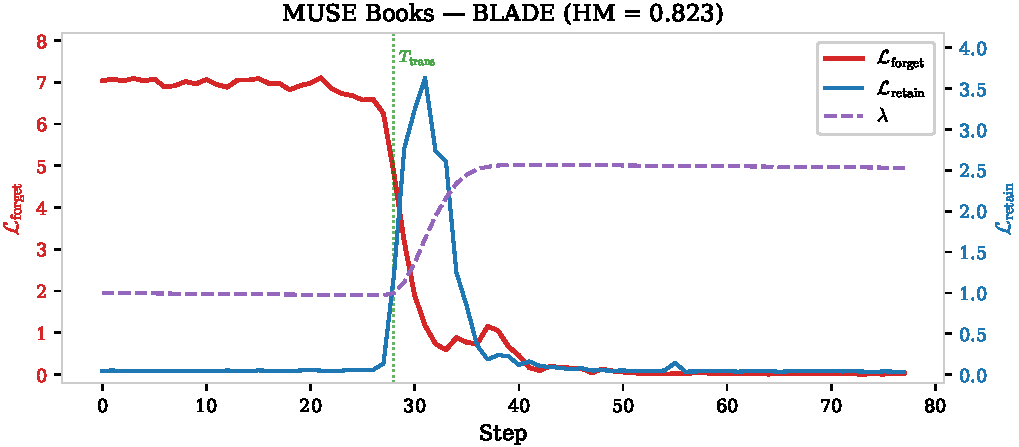
\includegraphics[width=\textwidth]{figures/fig_muse_books_dynamics.pdf}
        \caption{\method}
    \end{subfigure}
    \hfill
    \begin{subfigure}[t]{0.48\columnwidth}
        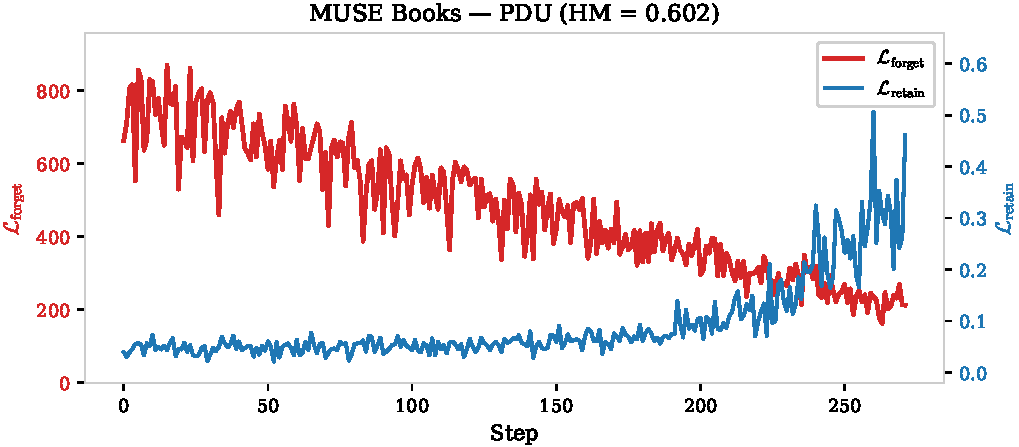
\includegraphics[width=\textwidth]{figures/fig_muse_books_PDU_dynamics.pdf}
        \caption{PDU}
    \end{subfigure}
    \caption{Training dynamics on MUSE Books. (a)~\method exhibits a three-phase pattern: warm-up $\to$ spike-and-ratchet $\to$ smooth convergence. The asymmetric $\lambda$ permanently ratchets up after the spike. (b)~PDU's unbounded loss produces recurring oscillations with no self-correction. Full results across all benchmarks in Appendix~\ref{app:dynamics}.}
    \label{fig:dynamics}
\end{figure}

\figref{fig:dynamics} illustrates the contrasting dynamics. \method follows a three-phase pattern across all benchmarks (Appendix~\ref{app:dynamics}):
(1)~\textbf{Warm-up}: forget loss declines steadily while retain stays near $\varepsilon$.
(2)~\textbf{Spike and ratchet}: accumulated forgetting disrupts shared representations, spiking retain loss; the asymmetric update ratchets $\lambda$ from ${\sim}1$ to 2.2--4.5, permanently elevating protection. The final $\lambda$ scales with task difficulty without hyperparameter change: 2.4 (fgt01) $\to$ 3.6 (fgt05) $\to$ 4.5 (fgt10).
(3)~\textbf{Smooth convergence}: the forget loss approaches zero with no further retain violations.

PDU shows qualitatively different behavior: its unbounded logit-margin loss starts at 700+ and produces recurring retain spikes throughout training. The symmetric dual update offers no lasting protection---$\lambda$ drops as fast as it rises, producing oscillatory cycles that never resolve.
